\documentclass[border=6pt]{standalone}
\usepackage{tikz}
\usetikzlibrary{arrows.meta,positioning,calc}
\begin{document}
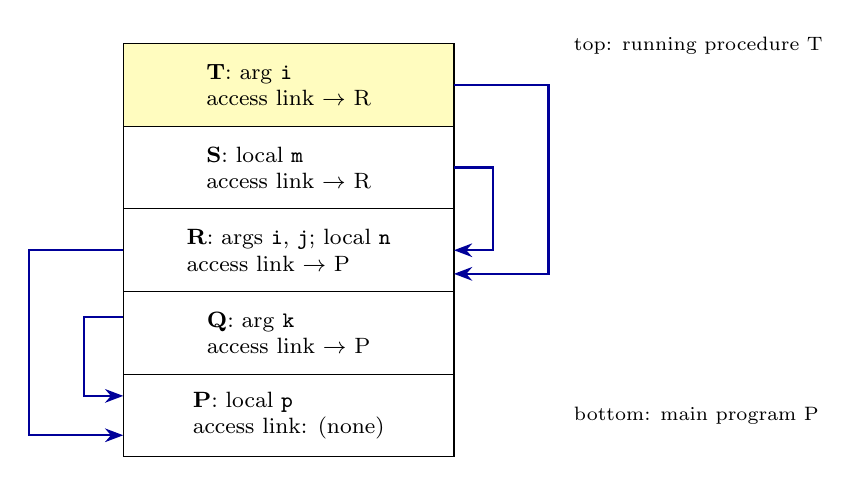
\begin{tikzpicture}[>=Stealth,font=\small,
  ar/.style={draw,minimum width=4.2cm,minimum height=1.05cm,align=left,font=\footnotesize,inner sep=3pt},
  lk/.style={->,thick,blue!60!black}]
\node[ar] (P) at (0,0) {\textbf{P}: local \texttt{p}\\ access link: (none)};
\node[ar] (Q) at (0,1.05) {\textbf{Q}: arg \texttt{k}\\ access link $\to$ P};
\node[ar] (R) at (0,2.1) {\textbf{R}: args \texttt{i}, \texttt{j}; local \texttt{n}\\ access link $\to$ P};
\node[ar] (S) at (0,3.15) {\textbf{S}: local \texttt{m}\\ access link $\to$ R};
\node[ar,fill=yellow!25] (T) at (0,4.2) {\textbf{T}: arg \texttt{i}\\ access link $\to$ R};
% links to P on the left
\draw[lk] (-2.1,1.25) -- (-2.6,1.25) -- (-2.6,0.25) -- (-2.1,0.25);
\draw[lk] (-2.1,2.1) -- (-3.3,2.1) -- (-3.3,-0.25) -- (-2.1,-0.25);
% links to R on the right
\draw[lk] (2.1,3.15) -- (2.6,3.15) -- (2.6,2.1) -- (2.1,2.1);
\draw[lk] (2.1,4.2) -- (3.3,4.2) -- (3.3,1.8) -- (2.1,1.8);
\node[font=\scriptsize,anchor=west] at (3.5,0) {bottom: main program P};
\node[font=\scriptsize,anchor=west] at (3.5,4.7) {top: running procedure T};
\end{tikzpicture}
\end{document}
